%--------------------------------------------------------------------------
\chapter{INTRODUCTION}

%--------------------------------------------------------------------------
\vspace{2em}
\setlength{\epigraphwidth}{0.86\textwidth}
\setlength{\epigraphrule}{0pt}
\epigraph{
	\textit{Music has become an almost arbitrary matter, and composers will no longer be bound by laws and rules, but avoid the names of School and Law as they would Death itself...}
}{-- Johann Joseph Fux}

%--------------------------------------------------------------------------
\section{Basic Derivation Techniques}

%--------------------------------------------------------------------------
Derivation is the process of extracting ordered segments from rows in order to generate new compositional materials. It is a technique that dates back to the Second Viennese School. Fig.~\ref{fig:schoenberg-quartet} shows an early example of this technique in Schoenberg's fourth string quartet \cite[100]{Westergaard1966}. In this example, the basic row is stated by the violins in the first bar shown, while combined with its $T_5I$ transform, which is presented by the viola and violoncello. In the second bar, this situation is reversed, and the violins present the $T_5I$ transform, while viola and violoncello state the $T_0$ transform.

%--------------------------------------------------------------------------
\begin{figure}[htbp]
    \centering
	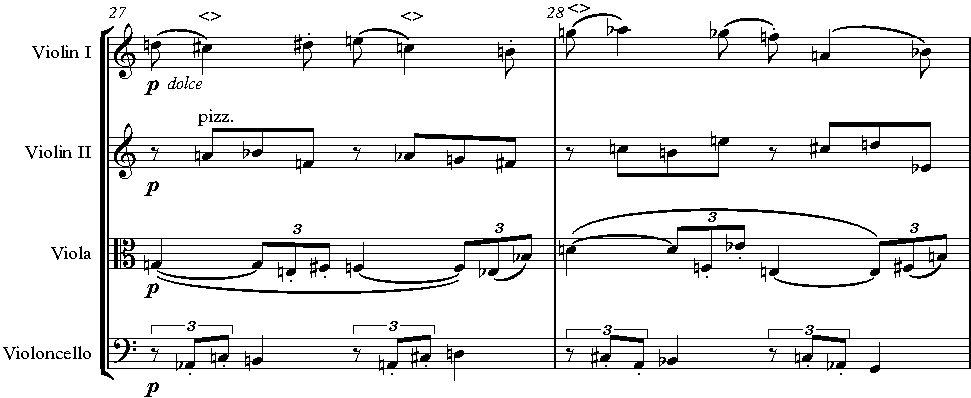
\includegraphics[width=6.5in]{figures/Schoenberg_4.pdf}
	\caption[Schoenberg's \emph{Fourth String Quartet} Op.~37]{Derived rows in Arnold Schoenberg's \emph{Fourth String Quartet} Op.~37 \cite[100]{Westergaard1966}.}
	\label{fig:schoenberg-quartet}
\end{figure}

%--------------------------------------------------------------------------
\noindent While separating the row between the two violins, two other rows are constructed, namely the row that is stated by the first violin between the two bars shown, and similarly the row that is stated by the second violin. These two rows are constructed from ordered segments extracted from the basic row, and so are said to be derived from it. Neither the first violin row, nor the second violin row are twelve-tone transforms of the original row or of each other. The same procedure of picking a fixed pattern of order numbers to separate the $[T_0 \; | \; T_5I]$ statement of the row between the two violins is used to split the $[T_5I \; | \; T_0]$ combined statement between viola and violoncello. While picking a fixed pattern of order numbers between the two lower instruments, however, the resulting linear statements for these instruments do not result in derived rows.

%--------------------------------------------------------------------------
Many structured approaches to derivation exist that guarantee that the extracted segments, when combined, will produce derived rows. These approaches often involve constructing a combination matrix of rows. The rows combined in the matrix are usually twelve-tone transforms of the same basic row. The rows that are derived from the segments of these transforms, on the other hand, may or may not be themselves transforms of the basic row.

%--------------------------------------------------------------------------
\begin{example}
The basic row in Berg's \emph{Lulu} may be used as motivation for a basic derivation procedure \cite[182]{Starr1984}. The first step is to create a $2 \times 24$ array where the first row $S$ is followed by $R(S)$, and the second row is initially undefined \cite[241]{Morris1977}.
\begin{equation}
    \left[
    \begin{array}{cccccccccccc|cccccccccccc}
    10 & 2 & 3 & 0 & 5 & 7 & 4 & 6 & 9 & 8 & 1 & 11 & 11 & 1 & 8 & 9 & 6 & 4 & 7 & 5 & 0 & 3 & 2 & 10 \\
    . & . & . & . & . & . & . & . & . & . & . & . & . & . & . & . & . & . & . & . & . & . & . & .
    \end{array}
    \right] \enspace.
\end{equation}
Next, an arbitrary segment is chosen, separated from the the top row, and placed in the bottom row.
\begin{equation}
    \left[
    \begin{array}{cccccccccccc|cccccccccccc}
    . & 2 & 3 & . & . & . & 4 & 6 & 9 & 8 & 1 & 11 & . & . & . & . & . & . & 7 & 5 & 0 & . & . & 10 \\
    10 & . & . & 0 & 5 & 7 & . & . & . & . & . & . & 11 & 1 & 8 & 9 & 6 & 4 & . & . & . & 3 & 2 & .
    \end{array}
    \right] \enspace.
\end{equation}
Let $V = \{ 2, 3, 4, 6, 9, 8, 1, 11, 7, 5, 0, 10 \}$. Then $V$ is a row derived from $S$. In particular, the ordered segment $\{ 10, 0, 5, 7 \}$ in $S$ is preserved by $R(V)$, and a counterpoint that combines $S$ vertically with $V$ horizontally is possible by construction.
\label{ex:derivation}
\end{example}

%--------------------------------------------------------------------------
\begin{figure}[htbp]
    \centering
	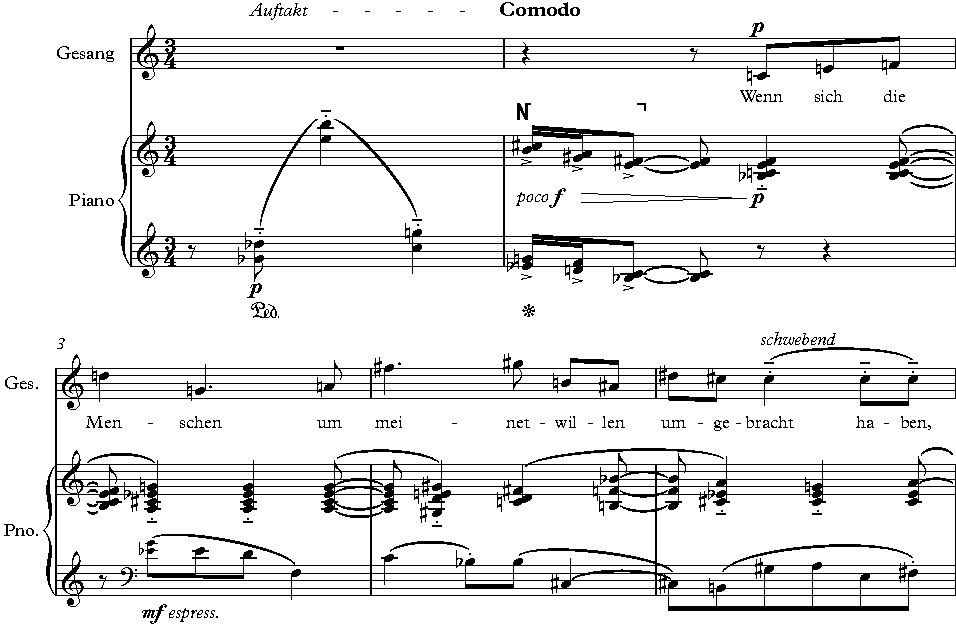
\includegraphics[width=6.5in]{figures/Berg_Lulu.pdf}
	\caption[Berg's \emph{Lied der Lulu}]{Alban Berg's \emph{Lied der Lulu} \cite[182]{Starr1984}.}
	\label{fig:berg-lulu}
\end{figure}

%--------------------------------------------------------------------------
It is of interest to note at this point that, in this kind of construction, the choice of a particular segment is already an important compositional decision. This choice bears relevance in that it establishes motivic material, that is, the segment itself. It also potentially introduces complementary harmonic regions, one given by the segment, the other given by its set complement. Moreover, and perhaps more importantly, it presents an opportunity for exploring syntax. There are a multitude of ways in which a composer may obtain syntax from a simple derivation procedure such as the one given in Ex.~\ref{ex:derivation}. One way would be to find an operation that makes the chosen segment invariant. In particular, it is easily checked that $S_1 = \{ 10, 0, 5, 7 \} = RT_5I(S_1)$. Ex.~\ref{ex:derivation} can then be followed by the combination matrix $[RT_5I(S) \; | \; T_5I(S_1)]$. In this second matrix, the segment $S_1$ could be preserved, but the row derived from $RT_5I(S)$ by preserving the segment $S_1$ would not be a transform of $V$. If the set complement of $S_1$ in $V$ were parsed to produce more than one harmonic region, then the complement of $S_1$ under this newly derived row would produce different harmonic regions under the same parsing. This procedure can be very pertinent compositionally, as it would be capable of producing contrasting harmonic regions while maintaining motivic coherence under the $S_1$ segment. Yet another way of generating syntax from derivation would be to follow $S$ with $V$ itself. A new row would then be derived from $V$, say $Q$, and eventually $V$ would be followed by $Q$. Repeating this procedure \emph{ad libitum} could generate many contrasting harmonic regions. In particular, this type of procedure is seen in Donald Martino's \emph{Notturno} of 1974, a composition that won the Pulitzer Prize in the following year \cite[181]{Starr1984}. If, by compositional choice, the same order numbers were always picked in the chain of derived rows, then a potential for rhythmic and agogic coherence could also be explored.

%--------------------------------------------------------------------------
\section{Literature Review}

%--------------------------------------------------------------------------
\enlargethispage{\baselineskip}
One of the earliest references in the academic literature of a procedure that may be construed as a derivation technique, illustrated below in Ex.~\ref{ex:martino-derivation}, is seen in \cite{Martino1961}, a paper whose main purpose is another, namely to generalize the construction of aggregate formations. The techniques described by Martino are influenced by Babbitt's ideas on combinatoriality \cite[224]{Martino1961}, and make extensive use of tables. In the interest of generalizing the construction of aggregate formations, Martino provides, in addition to hexachordal, also trichordal, tetrachordal, and even pentachordal combinatoriality tables, as well as somewhat brief discussions on oblique combinations \cite[241]{Martino1961}, which are further discussed in the context of derivation in \cite[216]{Starr1984}, and on uneven partitions of a row and their combinatoriality implications \cite[267]{Martino1961}. Martino acknowledges the aggregates formed by combinatoriality are not necessarily ordered, rather seeing this characteristic as capable of bringing harmonic diversity \cite[228, 230]{Martino1961}. In mentioning the derivation of new harmonic sets, this process is juxtaposed to another, namely the fragmentation of the original series. Both procedures are deemed to be essentially the same, since set derivation via aggregate formations can be seen as a fragmentation of the set obtained vertically \cite[230, 231]{Martino1961}.

%--------------------------------------------------------------------------
\begin{example}
	\label{ex:martino-derivation}
	\cite[231]{Martino1961}
	Let $S = \{ 0, 4, 11, 3, 1, 2, 5, 6, 9, 8, 10, 7 \}$ and consider the combination matrix $\hat{A}$.
	\begin{equation}
    	\hat{A} = [\hat{A}_1 | \hat{A}_2] = \left[
    	\begin{array}{cccccc|cccccc}
        	0 & 4 & 11 & 3 & 1 & 2 & 5 & 6 & 9 & 8 & 10 & 7 \\
        	7 & 10 & 8 & 9 & 6 & 5 & 2 & 1 & 3 & 11 & 4 & 0
    	\end{array}
    	\right] \enspace.
	\end{equation}
	In particular, the hexachords given by the $\hat{A}_i$ can be combined with their transforms under $T_1I$, yielding the combination matrix $A$.
	\begin{equation}
    	A = [A_1 | A_2 | A_3 | A_4] = \left[
    	\begin{array}{ccc|ccc|ccc|ccc}
        	0 & 4 & 11 & 3 & 1 & 2 & 5 & 6 & 9 & 8 & 10 & 7 \\
        	7 & 10 & 8 & 9 & 6 & 5 & 2 & 1 & 3 & 11 & 4 & 0 \\
        	\hline
        	1 & 9 & 2 & 10 & 0 & 11 & 8 & 7 & 4 & 5 & 3 & 6 \\
        	6 & 3 & 5 & 4 & 7 & 8 & 11 & 0 & 10 & 2 & 9 & 1
    	\end{array}
    	\right] \enspace.
	\end{equation}
	The row $Q = \{ 7, 0, 10, 6, 4, 1, 3, 5, 8, 9, 2, 11 \}$ can then be derived from the first column of $A$, but $T_9(Q)$ can only partially be derived from the second column of $A$, as pitch-classes 6 and 5 get swapped.
	\begin{equation}
        \left[
        \begin{array}{cccccccccccc|cccccccccccc}
            & 0 &&& 4 &&&&&&& 11 &&&& 3 & 1 &&& 2 &&&& \\
            7 && 10 &&&&&& 8 &&& && 9 &&&&&&& \boxed{6} & \boxed{5} && \\
            \hline
            &&&&& 1 &&&& 9 & 2 & &&&&&& 10 & 0 &&&& 11 & \\
            &&& 6 &&& 3 & 5 &&&& & 4 && 7 &&&&&&&&& 8
        \end{array}
        \right. \quad \cdots
    \end{equation}
\end{example}

%--------------------------------------------------------------------------
Even though the term derivation is not mentioned in \cite{Westergaard1966}, the paper introduces a mature conception of the problems involved with the technique of derivation. Two basic strategies for achieving polyphony from an essentially linear construct, namely partitioning and combining, are proposed \cite[95]{Westergaard1966}. Partitioning, which is illustrated in Fig.~\ref{fig:schoenberg-quartet}, consists of splitting a row into separate lines in a very Schenkerian fashion, with a bias toward partitioning the row in ways that preserve some of its intervallic structure \cite[100]{Westergaard1966}. Combining, on the other hand, departs from combination matrices, similarly to the technique demonstrated in Ex.~\ref{ex:martino-derivation}, and is truly remarkable in the sense that it already represents a technique for self-derivation \cite[101]{Westergaard1966}. Ex.~\ref{ex:westergaard} demonstrates the technique of combining.

%--------------------------------------------------------------------------
\enlargethispage{\baselineskip}
\begin{example}
	\label{ex:westergaard}
	\cite[102]{Westergaard1966}
	Let $S = \{ 2, 1, 9, 10, 5, 3, 4, 0, 8, 7, 6, 11 \}$ be a 12-tone row and consider the $12 \times 12$ matrix $A$.
	\begin{equation}
    	A = \left[
    	\begin{array}{cccccccccccc}
        	2 & 1 & 9 & 10 & 5 & 3 & 4 & 0 & 8 & 7 & 6 & 11 \\
        	1 & 0 & 8 & 9 & 4 & 2 & 3 & 11 & 7 & 6 & 5 & 10 \\
        	\vdots & \vdots & \vdots & \vdots & \vdots & \vdots & \vdots & \vdots & \vdots & \vdots & \vdots & \vdots \\
        	3 & 2 & 10 & 11 & 6 & 4 & 5 & 1 & 9 & 8 & 7 & 0
    	\end{array}
    	\right] \enspace.
	\end{equation}
	Then $\tilde{A}$ is a $12 \times 144$ combination matrix of self-derivation in which every column is a transform of $S$.
	\begin{equation}
    	\tilde{A} = \left[
    	\begin{array}{cccccccccccc|cccccccccccc|}
        	2 &&&&&&&&&&&    &  &&&&&&&& 1 &&& \\
        	& 1 &&&&&&&&&&   &  && 0 &&&&&&&&& \\
        	&&&&&&& 0 &&&&   &  &&& 11 &&&&&&&& \\
        	&&&&&&&&&&& 11   &  &&&&&&&&&&& 10 \\
        	&&& 10 &&&&&&&&  &  &&&&&&& 9 &&&& \\
        	&& 9 &&&&&&&&&   &  & 8 &&&&&&&&&& \\
        	&&&&&&&& 8 &&&   &  7 &&&&&&&&&&& \\
        	&&&&&&&&& 7 &&   &  &&&&& 6 &&&&&& \\
        	&&&&&&&&&& 6 &   &  &&&&&& 5 &&&&& \\
        	&&&& 5 &&&&&&&   &  &&&& 4 &&&&&&& \\
        	&&&&&& 4 &&&&&   &  &&&&&&&&&& 3 & \\
        	&&&&& 3 &&&&&&   &  &&&&&&&&& 2 &&
    	\end{array}
    	\; \quad \cdots \right. \enspace.
	\end{equation}
	The columns of $\tilde{A}$ are obtained by simply arranging the contents of each corresponding column of $A$. In particular, $\tilde{A} = [T_0(S) \; | \; T_5I(S) \; | \; \cdots$. Observing that 5 precedes 4 in the 10\textsuperscript{th} row of $\tilde{A}$, and similarly that 4 precedes 3 in the 11\textsuperscript{th} row of $\tilde{A}$, many alternative rearrangements of $\tilde{A}$ are possible, such as $\tilde{B}$.
	\pagebreak
	\begin{equation}
    	\tilde{B} = \left[
    	\begin{array}{cccccccccccc|cccccccccccc|}
        	2 &&&&&&&&&&&&&&&&&&&& 1 &&& \\
        	& 1 &&&&&&&&&&&&& 0 &&&&&&&&& \\
        	&& \vdots & \vdots &&&& \vdots & \vdots & \vdots & \vdots & \vdots & \vdots & \vdots && \vdots && \vdots & \vdots & \vdots &&&& \vdots \\
        	&&&& 5 && \boxed{4} &&&&&&&&&&&&&&&&& \\
        	&&&&&&&&&&&&&&&& \boxed{4} &&&&&& 3 & \\
        	&&&&& 3 &&&&&&&&&&&&&&&& 2 &&
    	\end{array}
    	\; \quad \cdots \right. \enspace.
    \end{equation}
    Combination matrices such as $A = [T_0 \; | \; \cdots \; | \; T_1]^T$ may be constructed in alternative ways where inverse and retrograde transforms of the row $S$ can be present. One possible sequence of transforms is
	\begin{equation}
		\{ T_0, T_{10}, T_{8}, T_{6}, T_{4}, T_{2}, T_{5}I, T_{3}I, T_{1}I, T_{11}I, T_{9}I, T_{7}I \} \enspace .
	\end{equation}
	Another is
	\begin{equation}
		\{ T_0, T_{8}, T_{4}, T_{11}I, T_{7}I, T_{3}I, RT_{9}, RT_{5}, RT_{1}, RT_{10}I, RT_{6}I, RT_{2}I \} \enspace .
	\end{equation}
\end{example}

%--------------------------------------------------------------------------
Self-derivation in $12 \times 144$ combination matrices is straightforward, since every column is capable of producing arbitrary transforms of any row. However, self-derivation in combination matrices of four rows or less is deemed more difficult to achieve in \cite[108]{Westergaard1966}. Although a systematic way to understand self-derivation in smaller combination matrices is not proposed in \cite{Westergaard1966}, the advancements in the field are extremely substantial and arguably one strong motivating force for the studies in self-derivation that follow in the subsequent decades.

%--------------------------------------------------------------------------
In one of the seminal academic works in the field of twelve-tone theory, \cite{Starr1984} utilizes a mostly set-theoretic framework to understand and categorize rows and procedures involved in producing combination matrices of derivation and self-derivation. This approach revolves around the idea of looking at sets from the standpoint of their order constraints: a totally constrained set with no precedence contradictions is a twelve-tone row; a completely unconstrained set of twelve tones represents the free aggregate; each column of the matrix $A$ in Ex.~\ref{ex:westergaard} is a free aggregate; a maximally constrained set corresponds to the simultaneous aggregate, that is, a twelve-tone cluster. Sets that live in-between can often be projected in the middle and background of a composition, a fact that here too contributes to a Schenkerian view of the technique of derivation \cite[183, 184]{Starr1984}. Mathematically, the ideas in \cite{Starr1984} translate into considering the set $U$ of all ordered pairs of pitch classes. There are twelve choices for the first position, and twelve choices for the second position. As both choices are independent, this set has cardinality $12^2 = 144$. An element of $U$ is called an order constraint, and a subset $C$ of $U$ is called a pitch-class relation. The latter can be viewed as a $12 \times 12$ matrix where the entry $c_{ij}$ is equal to one whenever $\{ i, j \} \in C$, and zero otherwise. Bitwise operations can be applied to these matrices in a very computationally efficient manner: bitwise \emph{and} and \emph{or} correspond respectively to set intersection and union. For any pair of pitch classes $x$ and $y$, define a relation $x \sim y$ on the power set of $U$ by the set inclusion of the element $\{ x, y \}$. A subset $C$ will then be reflexive if, whenever an element of $C$ (which is a set) contains the pitch class $x$, then $\{ x, x \} \in C$. In words, reflexivity means that if a reflexive collection $C$ of notes contains an element $x$, then $x$ precedes (and follows) itself in $C$. The free aggregate is a minimal reflexive subset of $U$ that contains all twelve tones. The relation $\sim$ will be symmetric if $\{ x, y \} \in C$ implies $\{ y, x \} \in C$, and antisymmetric whenever $\{ x, y \} \in C$ implies $\{ y, x \} \notin C$, for $x \ne y \in \mathbb{Z}/ 12 \mathbb{Z}$. Similarly, transitivity is defined as $\{ x, y \} \in C$ and $\{ y, z \} \in C$, then $\{ x, z\} \in C$; and trichotomy is defined as either $\{ x, y \} \in C$ or $\{ y, x \} \in C$ for any $x \ne y \in \mathbb{Z}/ 12 \mathbb{Z}$. The relation $\sim$ is, of course, an order relation on the set of twelve tones by definition. A partial order is one that is reflexive, transitive, and antisymmetric, while a total order (a row), is a partial order that satisfies trichotomy \cite[184, 185]{Starr1984}. Often, pitch-class relations will contain many redundancies due to transitivity. In order to express these relations as oriented graphs, such redundancies must first be removed, or pruned \cite[186]{Starr1984}. This process can be reversed and a pitch-class relation can be extended to the point of its transitive closure \cite[190]{Starr1984}. It is also common for a pitch-class relation to be absent of any order constraint involving both $\{ x, y \}$, in which case $x$ and $y$ are said to be incomparable. Such $x$ and $y$ are bound to be struck together, or else be linearized by the injection of some constraint that will make them comparable, as long as there still remains a partial order, that is, as long as this process does not introduce a symmetry, for instance. The set of all total orderings that can be linearized from some partial order is called its total order class \cite[188]{Starr1984}. In a completely analogous manner, a pitch-class relation can be can verticalized by removing constraints, and again minding that the result is still transitive and symmetric. A partial order covers another whenever the former is a verticalization of the latter. A simple procedure to guarantee that a verticalization will remain a partial order is to take its union with the free aggregate, then subject this union to an extension operation, thus providing reflexivity in the first step, as well as transitivity in the second \cite[192, 193]{Starr1984}. The following theorems provide more details on covering, as well as unions and intersections of pitch-class relations. In particular, Th.~\ref{starr-theorem} plays a crucial role in the construction of combination matrices of self-derivation from aggregate realizations \cite[222]{Starr1984}. Th.~\ref{starr-theorem-operations}, which is stated without proof, discusses aspects of applying twelve-tone operations to pitch-class relations.

%--------------------------------------------------------------------------
\begin{theorem}
    \cite[193]{Starr1984}
    \begin{enumerate}
        \item Covering is transitive;
        \vspace{-0.5em}
        \item A pitch-class relation is covered by its extension;
        \vspace{-0.5em}
        \item If a pitch-class relation covers another, then the extension of the former covers the extension of the latter.
    \end{enumerate}
\end{theorem}

%--------------------------------------------------------------------------
\begin{theorem}
    \cite[194]{Starr1984}
    \label{starr-theorem}
    Let $A$ and $B$ be partial orders and denote by $\Toc(A)$ and $\Toc(B)$ their respective total order classes. Then
    \begin{equation}
        \Toc(A) \cap \Toc(B) = \Toc(\Ext(A \cup B)) \enspace,
    \end{equation}
    where $\Ext$ is the extension operator. Moreover, if $A_i$ is a finite sequence of $n$ partial orders, then
    \begin{equation}
        \bigcap_{i = 0}^{n} \Toc(A_i) = \Toc \left[ \Ext\left ( \bigcup_{i = 0}^{n} A_i \right) \right] \enspace.
    \end{equation}
\end{theorem}

%--------------------------------------------------------------------------
\begin{theorem}
    \cite[194]{Starr1984}
    The intersection of two partial orders is again a partial order.
\end{theorem}

%--------------------------------------------------------------------------
\begin{theorem}
    \cite[195]{Starr1984}
    \label{starr-theorem-operations}
    Let $C$ be a pitch-class relation and $\{ a, b \}$ an element of $U$ such that $\{ a, b \} \in C$.
    \begin{enumerate}
        \item If $F$ is a pitch-class operation, then $\{ F(a), F(b) \} \in F(C)$ if and only if $\{ a, b \} \in C$. In particular, if $R(C)$ is the retrograde of $C$, then $\{ a, b \} \in R(C)$ if and only if $\{ b, a \} \in C$.
        \item If $C$ is totally ordered, then $R(C) = (S \setminus D) \cup F$, where $S$ is the simultaneous aggregate and $F$ is the free aggregate.
        \item If $C_1$ covers $C_2$, then $F(C_1)$ covers $F(C_2)$.
        \item Finally, if $C$ is $FR$-invariant, then all cycles in $F$ have length two.
    \end{enumerate}
\end{theorem}

%--------------------------------------------------------------------------
An aggregate realization is a particular type of partial order $C$ in which, for any pair of pitch classes $a, b$, if $a$ and $b$ are incomparable in $C$, then the set of pitch classes that precede $a$ in $C$ is equal to the set of pitch classes that precede $b$ in $C$, and also the set of pitch classes that follow $a$ in $C$ is equal to the set of pitch classes that follow $b$ in $C$. Aggregate realizations arise naturally from a total order in the sense that they belong to the set of all partial orders that are covered by this total order, and lead to a classification of partial orders, as well as to many musical applications. One interesting compositional application of aggregate realizations is that of projecting a total order as a middle-ground entity. Given a sequence $S$ of partial orders, all of which are covered by the same total order, say $X$, if both $X$ is never stated in the foreground and $S$ contains all order constraints in $X$, then a musical passage in which $S$ is stated in the foreground will bear $X$ as a middle-ground entity. In the case where $S$ does not comprise all the order constraints in $X$, some other partial order that covers $S$ will be projected in the middle-ground. In the particular case where a composer is dealing with pitch classes, projecting a partial order is equivalent to inducing the listener to infer its order constraints. If, in this case, two pitch classes are incomparable, then they are bound to be struck together \cite[197]{Starr1984}. Fig.~\ref{fig:webern-variations} shows Webern's Op.~27 opening bars and Ex.~\ref{ex:webern-variations} illustrates how an aggregate realization may be obtained from the first four bars therein \cite[203, 204]{Starr1984}. Whereas aggregate realizations correspond to a totally ordered sequence of disjoint subsets of the free aggregate, a columnar aggregate is, on the other hand, a set of disjoint row segments where, even though the internal order of each segment is total, all segments are pairwise incomparable. In addition, a columnar aggregate must contain the free aggregate as a subset, so that all pitch classes belonging to a given base are included in every column. The intersection of the set of all aggregate realizations with the set of all columnar realizations contains the set of all total orders (and thus all row segments), as well as the free aggregate. A total order is trivially an aggregate realization, and it is trivially a columnar realization. Any total order contains the free aggregate by the above \cite[201, 210]{Starr1984}.

%--------------------------------------------------------------------------
\enlargethispage{3em}
\begin{figure}[htbp]
    \centering
	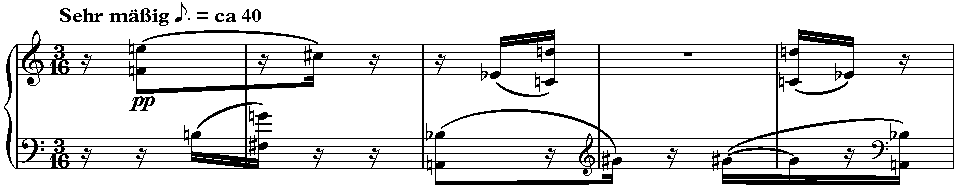
\includegraphics[width=6.5in]{figures/Webern_1.pdf}
	\caption[Webern's \emph{Variations for Piano} Op.~27]{Anton Webern's \emph{Variations for Piano} Op.~27 \cite[203]{Starr1984}.}
	\label{fig:webern-variations}
\end{figure}

%--------------------------------------------------------------------------
\begin{example}
    \cite[204]{Starr1984}
    \label{ex:webern-variations}
    Eq.~\ref{eq:webern-variations} shows an aggregate realization of Webern's Op.~27.
    \begin{equation}
    \label{eq:webern-variations}
    \begin{tikzcd}
		& E \arrow[dr] && G \arrow[dr] && B\flat \arrow[dr] && D \arrow[dr] & \\
		* \arrow[dr] \arrow[ur] && B \arrow[dr] \arrow[ur] && C\sharp \arrow[dr] \arrow[ur] && E\flat \arrow[dr] \arrow[ur] && G\sharp \\
		& F \arrow[ur] && F\sharp \arrow[ur] && A \arrow[ur] && C \arrow[ur] &
	\end{tikzcd}	
    \end{equation}
\end{example}

%--------------------------------------------------------------------------
A row segment is a pitch-class relation that is reflexive, transitive, and antisymmetric, with the additional requirement that some subset of its order constraints also satisfy trichotomy. Any partial order that covers some row segment is said to be an embedded segment of that partial order. By transitivity of covering, any other partial order covering the former partial order will have the aforementioned row segment embedded in it, including naturally any total order in its total order class. In this sense, a partial order may be seen as the union of its various embedded segments \cite[198]{Starr1984}. Row segments may be concatenated in a natural way. Let $X = \{ 0, 1, 2 \}$ and $Y = \{ 3, 4, 5 \}$ be row segments such that $X \cap Y = \emptyset$ when seeing $X$ and $Y$ as partial orders. The concatenation $X | Y$ will then be the partial order $X \cup Y \cup \{ \{ a, b \} : a \in X, b \in Y \}$. It follows both $X$ and $Y$ are embedded row segments of $X | Y$. The use of concatenation here is sequential, that is, the entire row segment $X$ precedes the entire row segment $Y$ in $X | Y$. In other words, intercalation of segments is not allowed when concatenating. Finding embedded segments that are common to different partial orders is straightforward. Let $X = \{ 0, 1, 7, 2, 10, 9, 11, 4, 8, 5, 3, 6 \}$ and $Y = \{ 1, 2, 8, 3, 11, 10, 0, 5, 9, 6, 4, 7 \}$ be total orders. In particular, $Y = T_1(X)$. Pruning the intersection $X \cap Y$ yields a graph whose longest row segments are $\{ 1, 2, 10, 9, 4 \}$, $\{ 1, 2, 10, 5, 6 \}$, $\{ 1, 2, 11, 5, 6 \}$, $\{ 1, 2, 8, 5, 6 \}$, and $\{ 1, 2, 8, 3, 6 \}$. These row segments are then the longest embedded segments of both $X$ and $Y$ \cite[200]{Starr1984}.

%--------------------------------------------------------------------------
Pruning an intersection of partial orders is also a method for computing common tones between sets that not only produces embedded segments, but can also be applied to the intersection of an arbitrary number of sets. When the sets are related to one another by a twelve-tone operation, finding common tones between them can be accomplished by expressing the operation as a permutation. Let $S = \{ 0, 1, 4, 5, 8, 9 \}$ and consider the cycle decomposition of $T_3I = (0 \; 3) \; (1 \; 2) \; (4 \; 11) \; (5 \; 10) \; (6 \; 9) \; (7 \; 8)$. It follows every pitch-class in $S$ maps to the twelve-tone complement of $S$ under $T_3I$. If the operation is $T_9 = (0 \; 9 \; 6 \; 3) \; (1 \; 10 \; 7 \; 4) \; (2 \; 11 \; 8 \; 5)$, then $S$ shares three common tones with $T_9(S)$, namely $0 \mapsto 9$, $4 \mapsto 1$, and $8 \mapsto 5$. A simple formula for computing the number of common tones between two sets under some $T_nI$ transform is also given in \cite[10]{Rahn1975}. Yet another technique for finding common tones between two sets consists of computing a table or matrix. This procedure has the advantage of not only giving all indices of transposition under which a set shares common tones with another, but of making it possible to determine whether these common tones will preserve their ordering after the transformation by examining the table's diagonals. It has the disadvantage of only being able to produce common tones between two sets at a time. Let $X$ be an $n$-tone row seen as a column vector, and consider the $n \times n$ matrix $A = [X, \cdots, X]$. In particular, the matrix $B = A - A^T$ will have a main diagonal of zeros, which indicates that $X$ shares with itself $n$ common tones under $T_0$. If there are $k$ threes in the matrix, then $X$ will share with itself $k$ tones under $T_3$. There is no requirement that a row be compared with itself. If, for instance, $A$ is given as above, and $\bar{A}$ is the matrix for the row $\bar{X}$, then counting the number $k$ of, say, threes in $B = A - \bar{A}^T$, will mean in turn that $X$ and $T_3(\bar{X})$ share $k$ tones under $T_3$. Naturally, the main diagonal of $B$ will not comprise only zeros if $A \ne \bar{A}$. To find common tones under inversion, let $B = A + A^T$ and, similarly, $M$ and $M \circ I$ become $B = A - M(A)^T$ and $B = A + M(A)^T$. Finally, if the indices being counted are disposed in any of the matrix's diagonals, then they will preserve ordering after the transform, thus becoming embedded segments; if, in addition, they are adjacent, then they will in fact be row segments shared by $X$ and the transform of $\bar{X}$ \cite[49]{Morris1987}. This matrix for finding common tones under transposition has the interesting property that it becomes a symmetric matrix when $A = \bar{A}$ and its elements are taken as interval classes. This reflects the fact that if $X$ shares $k$ tones with $T_i(X)$, then surely $T_i(X)$ will share exactly $k$ tones with $T_{12 - i}(X)$. If $i$ is an interval class, then $i = 12 - i$, showing why the matrix will be symmetric. The matrix of common tones under inversion is always symmetric, regardless whether its elements are taken as interval classes. Multiplicative operations, however, will often lack multiplicative inverses in twelve tones. For $p$-TET systems where $p$ is prime, multiplicative operations yield symmetric matrices as well, but those will sometimes require a proper definition of multiplicative interval classes.

%--------------------------------------------------------------------------
The procedure described in Ex.~\ref{ex:derivation} represents a type of derivation in which the series being displayed vertically is unrelated to the series being derived horizontally, except for the fact that both share a row segment when one of the rows is retrograded. The construction is part of a more general procedure, detailed in \cite[211]{Starr1984}, in which a row is always matched with a retrograded transform of itself. In the particular case of Ex.~\ref{ex:derivation}, the transform was $F = T_0$ for simplicity, but arbitrary twelve-tone operations may be used. Denote the given series by $S$ and define the derived row as $V = V_1 | V_2$, that is, $V$ is a concatenation of two row segments. The only requirement is that $V_1$, the segment that is singled out, remain invariant under $F$, which will force $V_2$ to also be invariant under $F$. In Ex.~\ref{ex:derivation} this requirement is satisfied trivially. It is usually the case in this type of derivation procedure that the invariance of $V$ under $F$, or under $R \circ F$ for that matter, does not preserve any ordering, as illustrated in Ex.~\ref{ex:derivation-unordered}. On the other hand, Ex.~\ref{ex:derivation-ordered} illustrates a derivation procedure similar to that in Ex.~\ref{ex:derivation} where the operation $F$ is not trivial and the singled-out segments are preserved as partial orders. That is accomplished by applying the technique described in \cite[49]{Morris1987} for finding common row segments. As a consequence of $F$ and the retrograde operation, combination matrices of this type feature two columns that are upside-down, $F$-mirrors of each other \cite[211]{Starr1984}. More can be said about such combination matrices. Prop.~\ref{derivation-polyphony-proposition} summarizes the general procedure under set-theoretic terms, and Eq.~\ref{eq:derivation-retrograde} provides the schematic representation of a derivation procedure involving the retrograde and an arbitrary operation $F$ \cite[212]{Starr1984}.

%--------------------------------------------------------------------------
\begin{proposition}
	\label{derivation-polyphony-proposition}
    \cite[211, 214]{Starr1984}
    Consider a 2-row combination matrix $C$ where a row is derived via the retrograde and some operation $F$. Denote the derived row by $V = V_1 | V_2$. Then the first column is the partial order $C_1 = V_1 \cup R \circ F(V_2)$, and similarly the second column is the partial order $C_2 = V_2 \cup R \circ F(V_1)$, such that $C_2 = R \circ F(C_1)$. If $D$ is a partial order that covers $C_1$, then $R \circ F(D)$ will cover $C_2$, and if $D$ is in the total order class of $C_1$, that is, $D$ is a row that can be linearized from $C_1$, then $R \circ F(D)$ is in the total order class of $C_2$. Finally, 2-row derivations of this type exist for arbitrary rows.
\end{proposition}

%--------------------------------------------------------------------------
\begin{equation}
\begin{array}{c|cc}
	\hline
    & S & R \circ F(S) \\
    \hline
    V & V_1 & V_2 \\
    R \circ F(V) & R \circ F(V_2) & R \circ F(V_1) \\
    \hline
\end{array}
\label{eq:derivation-retrograde}
\end{equation}

%--------------------------------------------------------------------------
\vspace{1em}
\begin{example}
    \cite[212]{Starr1984}
    \label{ex:derivation-unordered}
    Let $S = \{ 0, 1, 7, 2, 10, 9, 11, 4, 8, 5, 3, 6 \}$ and consider the operation $T_2I = (0 \; 2) \; (3 \; 11) \; (4 \; 10) \; (5 \; 9) \; (6 \; 8)$. Inspecting the cycle decomposition of $T_2I$ reveals that the segment $S_1 = \{ 0, 1, 7, 2 \}$ remains invariant under this operation. If a combination matrix involving $RT_2I$ is considered, however, then the segment $S_1$, seen as a partial order, shall not be preserved, since both $(1)$ and $(7)$ are fixed points. The same would happen to any $T_kI$ where $k$ is even. In particular, this shows that, in order to obtain the same ordered row segment in both columns of the combination matrix, $F$ cannot be trivial.
	\begin{equation}
    	\left[
    	\begin{array}{cccccccccccc|cccccccccccc}
        	0 & . & . & 1 & . & 7 & . & . & . & 2 & . & . & 10 & 9 & . & 11 & 4 & 8 & . & 5 & . & 3 & 6 & . \\
        	. & 8 & 11 & . & 9 & . & 6 & 10 & 3 & . & 5 & 4 & . & . & 0 & . & . & . & 7 & . & 1 & . & . & 2
    	\end{array}
    	\right] \enspace.
	\end{equation}
\end{example}

%--------------------------------------------------------------------------
\begin{example}
    \label{ex:derivation-ordered}
    Let $S = \{ 10, 2, 3, 0, 5, 7, 4, 6, 9, 8, 1, 11 \}$, the row in Berg's \emph{Lulu}, and consider the segment $\vec{s} = [10 \; 0 \; 5 \; 7]^T$ as a column vector. Now let $A^T = [\;\vec{s} \; | \; \vec{s} \; | \; \vec{s} \; | \; \vec{s}\;]$ be the square matrix whose every column is equal to $\vec{s}$. Then
	\begin{equation}
    	A + A^T = \begin{bmatrix}
    		2 & 10 & 3 & 5 \\
        	10 & 0 & 5 & 7 \\
        	3 & 5 & 10 & 0 \\
        	5 & 7 & 0 & 2
        \end{bmatrix} \pmod{12} \enspace.
	\end{equation}
	\noindent In particular, the row segment $\{ 10, 0, 5, 7 \}$ is invariant under $RT_5I$, since $A + A^T$ displays an anti-diagonal of fives. Thus, by matching $S$ with $RT_5I(S)$, the row segment $\{ 10, 0, 5, 7 \}$ may be obtained in the derived row $V$ itself, rather than in its retrograde, as was the case in Ex.~\ref{ex:derivation}. Setting it to $V_2$, say, yields $V = \{ 2, 3, 4, 6, 9, 8, 1, 11, 10, 0, 5, 7 \}$.
	\begin{equation}
    	\left[
    	\begin{array}{cccccccccccc|cccccccccccc}
        	. & 2 & 3 & . & . & . & 4 & 6 & 9 & 8 & 1 & 11 & . & . & . & . & . & . & 10 & 0 & 5 & . & . & 7 \\
        	10 & . & . & 0 & 5 & 7 & . & . & . & . & . & . & 6 & 4 & 9 & 8 & 11 & 1 & . & . & . & 2 & 3 & .
    	\end{array}
    	\right] \enspace.
	\end{equation}
\end{example}

%--------------------------------------------------------------------------
A distinction is made in \cite[211, 214]{Starr1984} between derivation and polyphonyzation. The former departs from a combination matrix of rows to infer a concatenation of rows that constitute the linearized result of flattening the combination matrix. The latter is the opposite concept, that is, given a concatenation of rows, a combination matrix is constructed such that each column breaks down the row at the top into disjoint ordered segments. Although differentiating between derivation and polyphonization is an important concept in the set-theoretic view of the problem, this paper shall not make that distinction. The term derivation will be used indiscriminately to both the breaking down of rows into contrapuntal combination matrices, and the flattening thereof.

%--------------------------------------------------------------------------
A related technique involving greater than 2-row counterpoint is achieved by folding a combination matrix. The process is similar to first constructing a matrix of hexachordal combinatoriality in the traditional sense, then deriving rows from this matrix using the techniques above. Let $S$ be a row whose first hexachord is invariant under the operation $G$. Consider a row $V = V_1 | V_2$ and an operation $F$ such that $S$ is in the total order class of $V_1 \cup R \circ F(V_2)$. Then putting $S$ in counterpoint with $G(S)$, as well as deriving $V$ from $S | R \circ F(S)$, yields the schematic representation in Eq.~\ref{eq:derivation-folded}. It is argued without proof that vertically satisfying $G$ while horizontally satisfying $F$ implies $F$ and $G$ must commute \cite[215]{Starr1984}. Ex.~\ref{ex:derivation-folded} shows an application of folded derivation.

%--------------------------------------------------------------------------
\pagebreak
\begin{equation}
\begin{array}{c|cc}
	\hline
	& S & R \circ F(S) \\
	\hline
	V & V_1 & V_2 \\
	R \circ F(V) & R \circ F(V_2) & R \circ F(V_1) \\
	R \circ GF(V) & R \circ GF(V_2) & R \circ GF(V_1) \\
	G(V) & G(V_1) & G(V_2) \\
	\hline
	& G(S) & R \circ GF(S) = R \circ FG(S) \\
	\hline 
\end{array}
\label{eq:derivation-folded}
\end{equation}

%--------------------------------------------------------------------------
\vspace{1em}
\begin{example}
    \cite[215]{Starr1984}
    \label{ex:derivation-folded}
    Let $S = \{ 0, 1, 11, 3, 8, 10, 4, 9, 7, 6, 2, 5 \}$ and consider the cycle decomposition of $T_6 = (0 \; 6) \; (1 \; 7) \; (2 \; 8) \; (3 \; 9) \; (4 \; 10) \; (5 \; 11)$. Let $V_1 = \{ 1, 3, 8, 9, 7, 2 \}$. Since the unordered set $V_1$ is $T_6$-invariant, it follows $V_2 = \{ 11, 0, 10, 4, 5, 6 \}$ and the following combination matrix is obtained:
    \begin{equation}
        \left[
        \begin{array}{cccccccccccc|cccccccccccc}
            & 1 && 3 & 8 &&& 9 & 7 && 2 && 11 && 0 &&& 10 & 4 &&& 5 && 6 \\
            0 && 11 &&& 10 & 4 &&& 6 && 5 && 8 && 1 & 3 &&& 2 & 9 && 7 &  
        \end{array}
        \right] \enspace.
    \end{equation}
    Consider further the cycle decomposition of $T_5I = (0 \; 5) \; (1 \; 4) \; (2 \; 3) \; (6 \; 11) \; (7 \; 10) \; (8 \; 9)$. Then $S_1 = \{ 0, 1, 11, 3, 8, 10 \}$ maps to its complement under $T_5I$, so $S$ can be used in a combination matrix where $S$ is matched with its transform under $T_5I$ in the usual way, that is, in a matrix of hexachordal combinatoriality. Moreover, the row $T_5I(V)$ can be derived from $T_5I(S)$. Since $T_5I$ commutes with $T_6$, as any pitch-class operation does, the following folded derivation is possible:
    \begin{equation}
        \left[
        \begin{array}{cccccccccccc|cccccccccccc}
            & 1 && 3 & 8 &&& 9 & 7 && 2 && 11 && 0 &&& 10 & 4 &&& 5 && 6 \\
            0 && 11 &&& 10 & 4 &&& 6 && 5 && 8 && 1 & 3 &&& 2 & 9 && 7 & \\
            \hline
            5 && 6 &&& 7 & 1 &&& 11 && 0 && 9 && 4 & 2 &&& 3 & 8 && 10 & \\
            & 4 && 2 & 9 &&& 8 & 10 && 3 && 6 && 5 &&& 7 & 1 &&& 0 && 11
        \end{array}
        \right] \enspace.
    \end{equation}
\end{example}

%--------------------------------------------------------------------------
\pagebreak
An analogue to the technique of oblique combination described in \cite[241, 267]{Martino1961} is given in \cite{Starr1984} in the context of folded derivation, and denoted skewed polyphonization. The procedure consists of shifting horizontally one of the two rows of the derivation matrix. Skewed polyphonization may be equivalent to folding combination matrices that involve the retrograde, and there is no requirement that the combinatoriality be hexachordal. Eq.~\ref{eq:derivation-shifted} provides a schematics description of a skewed polyphonization procedure involving the retrograde. The asterisk indicates there is no requirement that the same row class be derived in both foldings, in which case $V$ would be replaced by some other row $V^*$ and $G$ could be the identity. An interesting compositional application consists of matching altogether different foldings of a row, thus effectively bridging different derivations of the same generative material. Ex.~\ref{ex:derivation-shifted} shows an application of skewed polyphonization where combinatoriality is not hexachordal, but both foldings derive different transforms of the same row \cite[216]{Starr1984}.

%--------------------------------------------------------------------------
\begin{equation}
\begin{array}{c|ccc}
	\hline
    & S & R \circ F(S) & \\
    \hline
    V & V_1 & V_2 & \\
    R \circ F(V) & R \circ F(V_2) & R \circ F(V_1) & \\
    R \circ G(V)^* && R \circ G(V_2)^* & R \circ G(V_1)^* \\
    GF(V)^* && GF(V_1)^* & GF(V_2)^* \\
    \hline
    && GF(S) & R \circ G(S) \\
    \hline
\end{array}
\label{eq:derivation-shifted}
\end{equation}

%--------------------------------------------------------------------------
\vspace{1em}
\begin{example}
    \cite[216]{Starr1984}
    \label{ex:derivation-shifted}
    Consider the row $S = \{ 0, 1, 7, 2, 10, 9, 11, 4, 8, 5, 3, 6 \}$ and the combination matrix given by $RT_{10}I(S)$ against $T_{11}(S)$:
    \begin{equation}
        \left[
        \begin{array}{cccccccc|cccccccc}
            4 && 7 && 5 && 2 && 6 & 11 & 1 & 0 & 8 & 3 & 9 & 10 \\
            11 & 0 & 6 & 1 & 9 & 8 & 10 & 3 && 7 && 4 && 3 && 5
        \end{array}
        \right] \enspace.
    \end{equation}
    Deriving the row $V = V_1 | V_2 = \{ 1, 7, 2, 9, 8, 3 \} | \{ 4, 5, 6, 11, 0, 10 \}$ from $S | RT_{10}I(S)$, and following the scheme given in Eq.~\ref{eq:derivation-shifted}, yields the following shifted derivation:
    \pagebreak
    \begin{equation*}
        \left[
        \begin{array}{cccccccccccc|cccccccc|c}
            & 1 & 7 & 2 && 9 &&& 8 && 3 && 4 &&&& 5 &&&& 6 \\
            0 &&&& 10 && 11 & 4 && 5 && 6 & && 7 &&&& 2 && \\
            \hline
            &&&&&&&&&&&& & 0 & 6 & 1 && 8 &&& 7 \\
            &&&&&&&&&&&& 11 &&&& 9 && 10 & 3 &
        \end{array}
        \right. \quad \cdots
    \end{equation*}
    \begin{equation}
        \cdots \quad \left. \begin{array}{c|cccccccc|cccccccccccc}
            & 6 & 11 && 0 &&&& 10 &&&&&&&&&&& \\
            & && 1 && 8 & 3 & 9 & &&&&&&&&&&& \\
            \hline
            & 7 &&&& 3 &&& & 3 && 4 && 5 & 10 && 11 &&&& 9 \\
            3 &&& 4 &&&& 5 & && 6 && 1 &&& 0 && 7 & 2 & 8
        \end{array} \right] \enspace.
    \end{equation}
\end{example}

%--------------------------------------------------------------------------
\vspace{1em}
Self-derivation is discussed in \cite[217, 226]{Starr1984} both from the set-theoretic perspective, and from the standpoint of aggregate realizations. The only difference between self-derivation and the general case is that, in combination matrices of self-derivation, all row forms belong to the same row class, that is, all rows are $RT_nI$-transforms of the original row. The same applies to folded and skewed combination matrices of self-derivation. The general scheme for a two-row combination matrix of self-derivation involving the retrograde is given in Eq.~\ref{eq:derivation-self} \cite[219]{Starr1984}. It is stated without proof in \cite[217]{Starr1984} that the operations $F$ and $G$ in Eq.~\ref{eq:derivation-self} must commute. For this type of self-derivation on two-row counterpoint, however, simple inspection of the examples that follow such statement already affords a counter-proof, as described in Ex.~\ref{topSquareSideExample}. Similarly to the general derivation case, two-row self-derivations can also be folded. Although the same term is used, folding in combination matrices of self-derivation usually means taking one of the derived rows and pulling another level of self-derivation from it, as seen in Ex.~\ref{self-folded}. The problem size grows as a natural consequence of folding combination matrices of self-derivation. The folded rows can subsequently be folded, and this procedure can generate many levels of self-derivation \cite[221]{Starr1984}. Ex.~\ref{ex:scotto} provides a musical application of folded self-derivation matrices that constitute the main compositional procedure in Ciro Scotto's \emph{Tetralogy}. Folded self-derivation matrices are discussed in detail by Kowalski in \cite{Kowalski1987a}, always in the context of Eq.~\ref{eq:self-third} and not as the technique described in Ex.~\ref{ex:derivation-folded}.

%--------------------------------------------------------------------------
\begin{equation}
\begin{array}{c|cc}
	\hline
    & G(S) & R \circ FG(S) \\
    \hline
    S & S_1 & S_2 \\
    R \circ F(S) & R \circ F(S_2) & R \circ F(S_1) \\
    \hline
\end{array}
\label{eq:derivation-self}
\end{equation}

%--------------------------------------------------------------------------
\vspace{1em}
\begin{example}
	\label{topSquareSideExample}
    \cite[218]{Starr1984}
    Let $S = S_1 | S_2 = \{ 3, 8, 1, 0, 9, 6 \} | \{ 4, 7, 10, 5, 2, 11 \}$ and consider the cycle decomposition of $T_9I = (0 \; 9) \; (1 \; 8) \; (2 \; 7) \; (3 \; 6) \; (4 \; 5) \; (10 \; 11)$. In particular, both $S_1$ and $S_2$ are invariant under $T_9I$. It is not obvious, however, that $S$ and $RT_9I(S)$ can be derived from a combination matrix $A$ where the first column is $T_7(S)$ and the second is $RT_2I(S) = RT_9I \circ T_7(S)$. Here $F = T_9I$ and $G = T_7$. It is not the case that $F$ and $G$ commute, as $T_2I = F \circ G \ne G \circ F = T_4I$.
    \begin{equation}
    	\label{topSquareSideEquation}
        A = \left[
        \begin{array}{cccccccccccc|cccccccccccc}
            & 3 & 8 &&& 1 &&&& 0 & 9 & 6 &&&& 4 & 7 & 10 && 5 & 2 &&& 11 \\
            10 &&& 7 & 4 && 11 & 2 & 5 &&&& 3 & 0 & 9 &&&& 8 &&& 1 & 6 &
        \end{array}
        \right] \enspace.
    \end{equation}
\end{example}

%--------------------------------------------------------------------------
\begin{example}
    \cite[221]{Starr1984}
    \label{self-folded}
    Let $S = \{ 0, 11, 5, 10, 4, 2, 7, 9, 8, 3, 6, 1 \}$ and consider the following combination matrix given by $T_2(S) | RT_2(S)$, whose derived rows are $S$ and $R(S)$:
    \begin{equation}
        \label{eq:self-first}
        \left[
        \begin{array}{cccccccccccc|cccccccccccc}
            & 0 && 11 & 5 &&& 10 && 4 && 2 && 7 && 9 && 8 & 3 &&& 6 && 1 \\
            1 && 6 &&& 3 & 8 && 9 && 7 && 2 && 4 && 10 &&& 5 & 11 && 0 &
        \end{array}
        \right] \enspace.
    \end{equation}
    Subjecting the entire matrix to $T_1$ yields:
    \begin{equation}
        \label{eq:self-second}
        \left[
        \begin{array}{cccccccccccc|cccccccccccc}
            & 1 && 0 & 6 &&& 11 && 5 && 3 && 8 && 10 && 9 & 4 &&& 7 && 2 \\
            2 && 7 &&& 4 & 9 && 10 && 8 && 3 && 5 && 11 &&& 6 & 0 && 1 &
        \end{array}
        \right] \enspace.
    \end{equation}
    The entire matrix in Eq.~\ref{eq:self-first} can then be pulled from the first row of Eq.~\ref{eq:self-second}:
    \begin{equation}
    	\label{eq:self-third}
        \left[
        \begin{array}{cccccccccccc|cccccccccccc|c}
            &&& 0 &&&& 11 && 5 &&&&&& 10 &&& 4 &&&&& 2 & \\
            & 1 &&& 6 &&&&&&& 3 && 8 &&&& 9 &&&& 7 &&& 2 \\
            2 && 7 &&& 4 & 9 && 10 && 8 && 3 && 5 && 11 &&& 6 & 0 && 1 &&
        \end{array}
        \quad \cdots \right. \enspace.
    \end{equation}
\end{example}

%--------------------------------------------------------------------------
\begin{example}
    \cite[180]{Scotto2000}
    \label{ex:scotto}
    Let $S = \{ 0, 4, 7, 3, 11, 2, 10, 1, 6, 8, 9, 5 \}$ and consider the self-derivation array in Scotto's \emph{Tetralogy} given by Eq.~\ref{eq:scotto-1}. In it, the columns are $\{T_0 | RT_0\}$, and the derived rows are $\{T_7 | RT_7\}$.
    \begin{equation}
        \label{eq:scotto-1}
        \left[
        \begin{array}{cccccccccccc|cccccccccccc}
            && 7 && 11 & 2 & 10 && 6 && 9 && 5 && 8 && 1 &&&& 3 && 4 & 0 \\
            0 & 4 && 3 &&&& 1 && 8 && 5 && 9 && 6 && 10 & 2 & 11 && 7 &&
        \end{array}
        \right] \enspace.
    \end{equation}
	\noindent Similarly to Ex.~\ref{self-folded}, the above matrix can be folded in order to obtain subsequent levels of derivation. Unlike Ex.~\ref{self-folded}, however, Scotto derives a rotated transform of $S$ from $RT_7(S)$. The rows in Eq.~\ref{eq:scotto-folded} are thus $T_2(S), RT_2(S), \rho_6RT_2(S)$ and $\rho_6T_2(S)$, where $\rho$ is the cyclical rotation operator.
	\begin{equation*}
		\label{eq:scotto-folded}
        \left[
        \begin{array}{cccccccccccc|cccccccccccc|}
        	&&&&& 2 &&& 6 && 9 && 5 &&&& 1 &&&&&& 4 & \\
        	&& 7 && 11 && 10 &&&&&&&& 8 &&&&&& 3 &&& 0 \\
        	\hline
        	& 4 &&&&&& 1 &&&& 5 && 9 && 6 &&& 2 &&&&& \\
        	0 &&& 3 &&&&&& 8 &&&&&&&& 10 && 11 && 7 &&
        \end{array}
        \right. \quad \cdots
    \end{equation*}
	\begin{equation}
        \cdots \quad \left.
        \begin{array}{|cccccccccccc|cccccccccccc}
        	0 &&& 3 &&&&&& 8 &&&&&&&& 10 && 11 && 7 && \\
        	& 4 &&&&&& 1 &&&& 5 && 9 && 6 &&& 2 &&&&& \\
        	\hline
        	&& 7 && 11 && 10 &&&&&&&& 8 &&&&&& 3 &&& 0 \\
        	&&&&& 2 &&& 6 && 9 && 5 &&&& 1 &&&&&& 4 &
        \end{array}
        \right] \enspace.
    \end{equation}
	\noindent In an entirely Schenkerian fashion, Scotto utilizes the folded array as the source material for the middle-ground structure of \emph{Tetralogy}. The only difference between the derivation array and the Schenkerian graph is that $T_2(S)$ now corresponds to the alto register, as seen in Fig.~\ref{fig:scotto-schenker1}. One of the foreground realizations of the Schenkerian graph in Fig.~\ref{fig:scotto-schenker1} is given in Fig.~\ref{fig:scotto-music1}. Rather than a strict serial composition, \emph{Tetralogy} employs a variety of prolongation procedures which are in line with its Schenkerian orientation.
	\begin{figure}[H]
    	\centering
		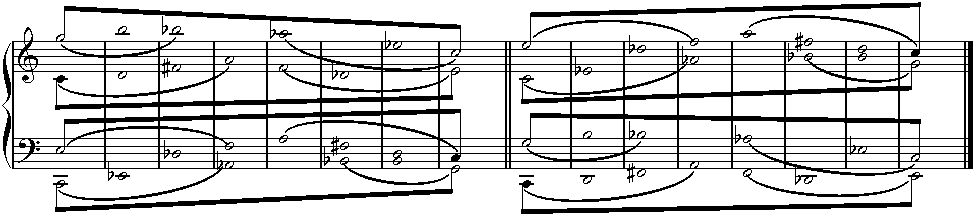
\includegraphics[width=6.5in]{figures/Scotto_Schenker_1.pdf}
		\caption[Schenkerian middle-ground structure in Scotto's \emph{Tetralogy}]{Schenkerian middle-ground structure in Scotto's \emph{Tetralogy}.}
    	\label{fig:scotto-schenker1}
	\end{figure}
	\begin{figure}[H]
    	\centering
    	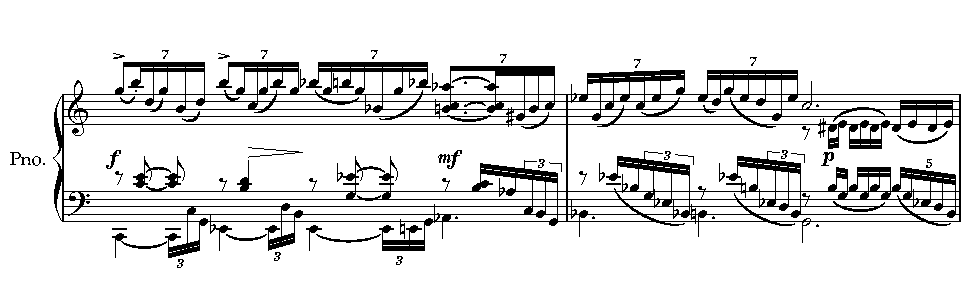
\includegraphics[width=6.5in]{figures/Scotto_1.pdf}
		\caption[Musical realization of the middle-ground in Scotto's \emph{Tetralogy}]{Musical realization of the middle-ground in Scotto's \emph{Tetralogy}.}
    	\label{fig:scotto-music1}
	\end{figure}
	\noindent The idea of prolongation in \emph{Tetralogy} extends beyond the foreground musical surface, and is applied as well to the middle-ground structure itself, effectively pushing it further into the background of the piece. The prolongation of the first bar in Fig.~\ref{fig:scotto-schenker1} is depicted in Fig.~\ref{fig:scotto-schenker2}, and a musical realization thereof is displayed in Fig.~\ref{fig:scotto-music2}. 
	\begin{figure}[H]
    	\centering
    	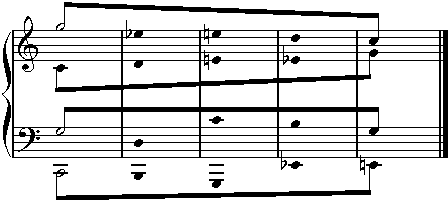
\includegraphics[width=3in]{figures/Scotto_Schenker_2.pdf}
    	\caption[Prolongation of the middle-ground structure in Scotto's \emph{Tetralogy}]{Prolongation of the middle-ground structure in Scotto's \emph{Tetralogy}.}
    	\label{fig:scotto-schenker2}
	\end{figure}
	\begin{figure}[H]
    	\centering
    	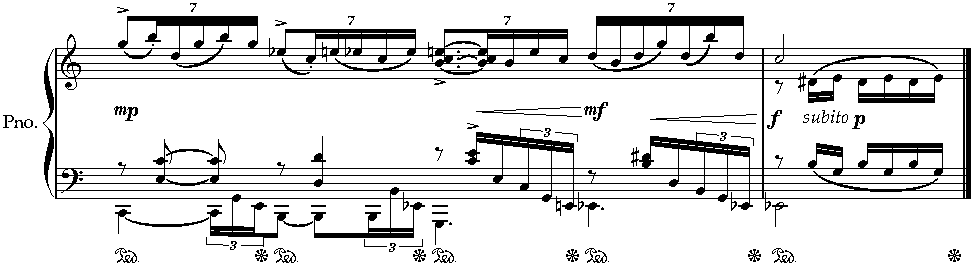
\includegraphics[width=6.5in]{figures/Scotto_2.pdf}
    	\caption[Musical realization of the prolonged middle-ground in Scotto's \emph{Tetralogy}]{Musical realization of the prolonged middle-ground in Scotto's \emph{Tetralogy}.}
    	\label{fig:scotto-music2}
	\end{figure}
\end{example}

%--------------------------------------------------------------------------
Three algorithms for computing combination matrices of self-derivation are presented in \cite{Starr1984}. The first is an algorithm for computing $2 \times 24$ matrices that consists of finding a segment at the beginning of an ordered set that can become an embedded segment in some transform of the set, then constructing a combination matrix involving the retrograde by manually resolving any symmetries. There is no prior knowledge of the entire row, thus the row is actually composed by adding order constraints to an initially unconstrained set \cite[217]{Starr1984}. The second algorithm utilizes Th.~\ref{starr-theorem} to construct self-derivation from columnar aggregates by finding operations that resolve symmetries between the columns of the matrix. Although there is no requirement that the matrix be retrograde-invariant, the retrograde makes it arguably easier to work out the algorithm by hand. Ex.~\ref{ex:starr-algorithm-2} illustrates the second algorithm in which, similarly to the first, the entire row is discovered as a result of the procedure \cite[222]{Starr1984}. The third algorithm proposed makes use of aggregate realizations to compose combination matrices of self-derivation, and also utilizes Th.~\ref{starr-theorem}. Ex.~\ref{ex:starr-aggregate-realization} illustrates how this third algorithm works by explicitly building the aggregate realizations in the matrix from the cycles of some operation \cite[226, 227]{Starr1984}, and Ex.~\ref{ex:stingray} shows how a $6 \times 72$ matrix of self-derivation may be used in a musical composition. This matrix was constructed by exploring the symmetries of an aggregate realization, that is, by using the third algorithm described in \cite{Starr1984}.

%--------------------------------------------------------------------------
\pagebreak
\begin{example}
	\cite[224]{Starr1984}
	\label{ex:starr-algorithm-2}
    Let $S = \{ 0, 1, 7, 2 \} | \{ 10, 9 \} | \{ 11, 4, 8, 5 \} | \{ 3, 6 \}$. Given that the complement of a row's first hexachord is always obtained from its second hexachord, a trivial case of hexachordal combinatoriality results when a row is matched with its retrograde. It is then possible to partition $S$ such that the combination matrix will have four columns:
    \begin{equation}
        A = \left[
        \begin{array}{c|c|c|c}
        	\{ 0, 1, 7, 2 \} & \{ 10, 9 \} & \{ 11, 4, 8, 5 \} & \{ 3, 6 \} \\
        	\{ 6, 3 \} & \{ 5, 8, 4, 11 \} & \{ 9, 10 \} & \{ 2, 7, 1, 0 \}
        \end{array}
        \right] \enspace.
    \end{equation}
    Now consider the cycles of $T_{11}I = (0 \; 11) \; (1 \; 10) \; (2 \; 9) \; (3 \; 8) \; (4 \; 7) \; (5 \; 6)$. In particular, the first column of $A$ will comprise the partial order $S_1 \cup R(S_4)$, and this union will, in turn, map onto its hexachordal complement under $T_{11}I$, as it takes precisely one element from each of the operation's cycles, all of which have length two. Since the second column above is the complement of the first, it will also map onto its complement under $T_{11}I$. Because the third and fourth columns are mirrors of the first two, hexachordal combinatoriality under $T_{11}I$ is obtained in every column, that is, for the partial orders $S_1 \cup R(S_4)$ and $S_2 \cup R(S_3)$, as well as their retrogrades. The same result is not obtained between $S$ and $T_{11}I(S)$, that is, the first hexachord of $T_{11}I(S)$ is \emph{not} the complement of the first hexachord of $S$. This procedure yields the matrix $\hat{A}$.
    \begin{equation}
        \hat{A} = \left[
        \begin{array}{c|c|c|c}
        	\{ 0, 1, 7, 2 \} & \{ 10, 9 \} & \{ 11, 4, 8, 5 \} & \{ 3, 6 \} \\
        	\{ 6, 3 \} & \{ 5, 8, 4, 11 \} & \{ 9, 10 \} & \{ 2, 7, 1, 0 \} \\
        	\{ 11, 10, 4, 9 \} & \{ 1, 2 \} & \{ 0, 7, 3, 6 \} & \{ 8, 5 \} \\
        	\{ 5, 8 \} & \{ 6, 3, 7, 0 \} & \{ 2, 1 \} & \{ 9, 4, 10, 11 \}
        \end{array}
        \right] \enspace.
    \end{equation}
    The above can be construed as a sequence of four columnar aggregates. It may be possible to derive members of the same row class from each column. If the total order class of the intersection of all columns is not empty, that is, if it contains the free aggregate and does not contain any symmetry, then Th.~\ref{starr-theorem} guarantees that representatives of this row class can be derived from each column. Let $C_1, C_2, C_3, C_4$ be the four columns of the matrix $\hat{A}$. It follows the row $V = \{ 11, 0, 1, 6, 10, 4, 7, 2, 9, 5, 3, 8 \}$ has the property that $T \in \Toc \{ \Ext[ C_1 \cup RT_1I(C_2) \cup T_1I(C_3) \cup R(C_4) ] \}$. Therefore $[V | RT_1I(V) | T_1I(V) | R(V)]$ can be derived from the columns of $\hat{A}$.
    \begin{equation*}
        \left[
        \begin{array}{cccccccccccc|cccccccccccc|}
            & 0 & 1 &&&& 7 & 2 &&&& && 10 &&&&& 9 &&&&& \\
            &&& 6 &&&&&&& 3 & & 5 && 8 & 4 & 11 &&&&&&& \\
            \hline
            11 &&&& 10 & 4 &&& 9 &&& &&&&&&&&&&& 1 & 2 \\
            &&&&&&&&& 5 && 8 &&&&&& 6 && 3 & 7 & 0 &&
        \end{array}
        \right. \quad \cdots
    \end{equation*}
    \begin{equation}
        \cdots \left. \quad
        \begin{array}{|cccccccccccc|cccccccccccc}
            &&&&&&& 11 & 4 & 8 && 5 && 3 &&&&&&& 6 &&& \\
            &&&&& 9 &&&&& 10 & &&&&& 2 & 7 &&&& 1 & 0 & \\
            \hline
            && 0 & 7 & 3 && 6 &&&&& & 8 && 5 &&&&&&&&& \\
            2 & 1 &&&&&&&&&& &&&& 9 &&& 4 & 10 &&&& 11
        \end{array} \right] \enspace.
    \end{equation}
\end{example}

%--------------------------------------------------------------------------
\begin{example}
    \cite[226, 227]{Starr1984}
    \label{ex:starr-aggregate-realization}
    Let
    \begin{equation}
    	S = S_1 \; | \; S_2 \; | \; S_3 = \{ 0, 1, 7, 2 \} \; | \; \{ 10, 9, 11, 4 \} \; | \; \{ 8, 5, 3, 6 \}
    \end{equation}
    and consider the matrix $A = [S \; | \; T_4(S) \; | \; T_8(S)]^T$.
    \begin{equation}
        A = \left[
        \begin{array}{cccc|cccc|cccc}
        	0 & 1 & 7 & 2 & 10 & 9 & 11 & 4 & 8 & 5 & 3 & 6 \\
        	4 & 5 & 11 & 6 & 2 & 1 & 3 & 8 & 0 & 9 & 7 & 10 \\
        	8 & 9 & 3 & 10 & 6 & 5 & 7 & 0 & 4 & 1 & 11 & 2
        \end{array}
        \right] \enspace.
    \end{equation}
    Now let $V$ be in the total order class of the first columnar aggregate of $A$. Next, rewrite the first columnar aggregate of $A$ as the aggregate realization $A_1$.
    \begin{equation}
        A_1 = \begin{tikzcd}
            & 0 \arrow[dr] && 1 \arrow[dr] && 7 \arrow[dr] && 2 \arrow[dr] & \\
            * \arrow[r] \arrow[dr] \arrow[ur] & 4 \arrow[r] & * \arrow[r] \arrow[dr] \arrow[ur] & 5 \arrow[r] & * \arrow[r] \arrow[dr] \arrow[ur] & 11 \arrow[r] & * \arrow[r] \arrow[dr] \arrow[ur] & 6 \arrow[r] & * \\
            & 8 \arrow[ur] && 9 \arrow[ur] && 3 \arrow[ur] && 10 \arrow[ur] &
        \end{tikzcd}
    \end{equation}
    When the first column of $A$ is regarded as an aggregate realization, it becomes clearer that any $V \in \Toc(A_1)$ must be a succession of augmented triads. One possibility would be $V = \{ 4, 8, 0, 9, 1, 5, 11, 7, 3, 2, 10, 6 \}$. It is easy to see that linearizing $V$ from $A_1$ is possible, but it is not obvious whether some transform of $V$ can be linearized from the other columns of $A$. The answer depends on the chosen operation, $T_4$ in this case, and on the chosen $S$. To verify that $A_2$ is a transform of $A_1$, it suffices to check whether there is a base-four $RT_nMI$ operation that maps $S_1 \pmod 4$ onto $S_2 \pmod 4$. This is easily verified, as indeed
    \begin{equation}
        S_1 \pmod 4 = \{ 0, 1, 3, 2 \} = T_2I(\{ 2, 1, 3, 0 \}) = T_2I \circ S_2 \pmod 4 \enspace.
    \end{equation}
    The above method works because the elements in each of $A_1$'s columns are incomparable, thus may be picked from each column in any order. In other words, $A_1$ could be flipped horizontally, say, and still have the same aggregate realization. Since all of $A$'s columns can be reduced $\mod 4$ by construction, it becomes enough to only consider each column's residue modulo four, and four-tone operations. Since $S_1 \pmod 4 = S_3 \pmod 4$, $V$ itself can be derived from $A_3$, yielding the following derivation matrix, where the second column is $T_2I(V)$:
    \begin{equation*}
        \left[
        \begin{array}{cccccccccccc|cccccc}
        	&& 0 && 1 &&& 7 && 2 && & 10 &&&&& 9 \\
        	4 &&&&& 5 & 11 &&&&& 6 & && 2 && 1 & \\
        	& 8 && 9 &&&&& 3 && 10 & & & 6 && 5 &&
        \end{array}
        \right. \quad \cdots
    \end{equation*}
    \begin{equation}
        \cdots \left. \quad
        \begin{array}{cccccc|cccccccccccc}
        	&& 11 && 4 & & & 8 &&&& 5 &&& 3 &&& 6 \\
        	3 &&&&& 8 & && 0 & 9 &&&& 7 &&& 10 & \\
        	& 7 && 0 && & 4 &&&& 1 && 11 &&& 2 &&
        \end{array}
        \right] \enspace.
    \end{equation}
    It may be possible to derive other rows from $A$ that are not based on the concatenation of cycles from an operation. Knowing that the columns of $A$ are related as aggregate realizations by the operation tuple $\mathcal{A} = [T_0 \; T_2I \; T_0]$, and regarding the $A_i$ as columnar aggregates, take $\hat{A} = \Ext[\bigcup_i(\mathcal{A}_i \circ A_i)]$. By Th.~\ref{starr-theorem}, any row that can be linearized from $\hat{A}$, will be in $\bigcap_i \Toc(A_i)$, and thus its $\mathcal{A}_i$-transform can be derived from each $i$-column of $A$. Below is the columnar aggregate $\hat{A}$.
    \begin{equation}
        \hat{A} = \begin{tikzcd}
            & 0 \arrow[r] \arrow[ddr] & 1 \arrow[r] \arrow[dr] & 7 \arrow[r] \arrow[ddr] & 2 \arrow[dr] & \\
            * \arrow[r] \arrow[dr] \arrow[ur] & 4 \arrow[r] \arrow[ur] & 5 \arrow[r] \arrow[dr] & 11 \arrow[r] \arrow[ur] & 6 \arrow[r] & * \\
            & 8 \arrow[r] \arrow[ur] & 9 \arrow[r] \arrow[uur] & 3 \arrow[r] \arrow[ur] & 10 \arrow[ur] &
        \end{tikzcd}
    \end{equation}
    It follows $\hat{V} = \{ 0, 1, 4, 8, 9, 5, 7, 2, 11, 3, 10, 6 \}$ can be linearized from $\hat{A}$, yielding the derivation matrix below:
    \begin{equation*}
        \left[
        \begin{array}{cccccccccccc|cccccc}
        	0 &&&& 1 & 7 &&& 2 &&&&&&& 10 && \\
        	&&& 4 &&& 5 & 11 &&& 6 && 2 &&&& 1 & \\
        	& 8 & 9 &&&&&&& 3 && 10 && 6 & 5 &&& 7
        \end{array}
        \right. \quad \cdots
    \end{equation*}
    \begin{equation}
        \cdots \left. \quad
        \begin{array}{cccccc|cccccccccccc}
        	9 &&& 11 && 4 && 8 &&&&& 5 &&& 3 & 6 & \\
        	& 3 &&& 8 && 0 && 9 &&& 7 &&&&&& 10 \\
        	&& 0 &&&&&&& 4 & 1 &&& 11 & 2 &&&
        \end{array}
        \right] \enspace.
    \end{equation}
\end{example}

%--------------------------------------------------------------------------
\begin{example}
    \label{ex:stingray}
    Consider the aggregate realization A.
    \begin{equation}
        A = \begin{tikzcd}
            & 0 \arrow[dddr] && 1 \arrow[dddr] & \\
            & 4 \arrow[ddr] && 5 \arrow[ddr] & \\
            & 8 \arrow[dr] && 9 \arrow[dr] & \\
            * \arrow[ur] \arrow[uur] \arrow[uuur] \arrow[dr] \arrow[ddr] \arrow[dddr] && * \arrow[ur] \arrow[uur] \arrow[uuur] \arrow[dr] \arrow[ddr] \arrow[dddr] && * \\
            & 11 \arrow[ur] && 10 \arrow[ur] & \\
            & 7 \arrow[uur] && 6 \arrow[uur] & \\
            & 3 \arrow[uuur] && 2 \arrow[uuur] &
        \end{tikzcd}
    \end{equation}
    It is easily seen that $A$ is invariant under the set of operations $\Omega = \{ T_0, T_4, T_8, T_3I, T_7I, T_{11}I \}$. Thus if $\rho \in \Toc(A)$, then also $\Omega_i(\rho) \in \Toc(A)$. It is also easy to see that $R(\rho) \in \Toc(R \circ \Omega_i(A))$. Now let $S = \{ 0, 1, 5, 8, 9, 4, 10, 3, 7, 6, 2, 11 \}$, and consider the combination matrix $\mathcal{A} = [\mathcal{A}_1 | \cdots | \mathcal{A}_6]$.
    \begin{equation}
        \mathcal{A} = \left[
        \begin{array}{cc|cc|cc|cc|cc|cc}
            0 & 1 & 5 & 8 & 9 & 4 & 10 & 3 & 7 & 6 & 2 & 11 \\
            4 & 5 & 9 & 0 & 1 & 8 & 2 & 7 & 11 & 10 & 6 & 3 \\
            8 & 9 & 1 & 4 & 5 & 0 & 6 & 11 & 3 & 2 & 10 & 7 \\
            11 & 10 & 6 & 3 & 2 & 7 & 1 & 8 & 4 & 5 & 9 & 0 \\
            7 & 6 & 2 & 11 & 10 & 3 & 9 & 4 & 0 & 1 & 5 & 8 \\
            3 & 2 & 10 & 7 & 6 & 11 & 5 & 0 & 8 & 9 & 1 & 4
        \end{array}
        \right] \enspace.
    \end{equation}
    By construction, every row of $\mathcal{A}$ is an $\Omega$-transform of $S$. Also by construction, every $\mathcal{A}_i$ is an instance of either $A$ or $R(A)$, seen as a columnar aggregate, and thus $\Omega$-invariant. It follows a transform of $S$ can be derived from every $\mathcal{A}_i$. Since $T_7(S) \in \Toc(\mathcal{A}_1)$ and $RT_0I(S) \in \Toc(\mathcal{A}_2)$, the self-derivation matrix $X$ is obtained.
    \begin{equation}
        X = \left[
        \begin{array}{cccccccccccc|cccccccccccc}
            &&&&& 11 && 10 &&&&&&& 6 &&&&& 3 &&&& \\
            &&&& 4 && 5 &&&&&&&&&& 9 &&&&&&& 0 \\
            &&& 3 &&&&& 2 &&&&& 10 &&&&&&&& 7 && \\
            && 0 &&&&&&& 1 &&&&&& 5 &&& 8 &&&&& \\
            & 8 &&&&&&&&& 9 && 1 &&&&&&&& 4 &&& \\
            7 &&&&&&&&&&& 6 &&&&&& 2 &&&&& 11 &
        \end{array}
        \right] \enspace.
    \end{equation}
    It is important to point out that, although the matrix $X$ could be extended to a $6 \times 72$ derivation matrix wherein all columns of $\mathcal{A}$ are presented, this could not be done using arbitrary transforms of $S$. Upon inspection, it follows that the transforms of $S$ that can be derived from $\mathcal{A}_1$ and $\mathcal{A}_5$ are in
    \begin{equation}
        \{ T_3, T_7, T_{11}, RT_1, RT_5, RT_9, T_0I, T_4I, T_8I, RT_2I, RT_6I, RT_{10}I \} \enspace.
    \end{equation}
    For the columns $\mathcal{A}_2, \mathcal{A}_3, \mathcal{A}_4$ and $\mathcal{A}_6$, the transforms of $S$ that can be derived are in
    \begin{equation}
        \{ T_1, T_5, T_9, RT_3, RT_7, RT_{11}, T_2I, T_6I, T_{10}I, RT_0I, RT_4I, RT_8I \} \enspace.
    \end{equation}
    Rather than a hinderance, this fact can be leveraged to explore contrasting harmonic regions. Fig.~\ref{fig:stingray} shows a musical realization of $X$:
    \begin{figure}[htbp]
        \centering
        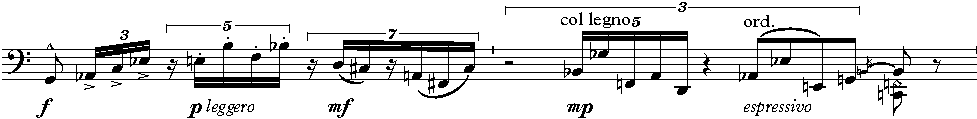
\includegraphics[width=6.5in]{figures/stingray-example.pdf}
        \caption[Self-derivation in Damiani's \emph{Variations for Violoncello}.]{Self-derivation in Damiani's \emph{Variations for Violoncello}.}
        \label{fig:stingray}
    \end{figure}
\end{example}

%--------------------------------------------------------------------------
The framework provided by \cite{Starr1984} is expanded in \cite{Kowalski1987a}, a paper that focuses mostly on the problem of self-derivation. In particular, this focus is restricted to combination matrices with problem sizes two and three, as larger problem sizes are deemed increasingly straightforward to achieve. The technique of folding, as illustrated in Ex.~\ref{self-folded}, is discussed in depth and presented as an alternative to achieving larger than $2 \times 24$ combination matrices \cite[298]{Kowalski1987a}. The direction taken in \cite{Kowalski1987a} differs substantially from \cite{Starr1984} not only in the sense that the former does not stress derivation in general, but also because it constantly emphasizes qualitative aspects of self-derivation. Arguably the greatest contribution in that regard is the introduction of the concept of \emph{merge index} in combination matrices of self-derivation. The merge index measures how row segments are interweaved in a combination matrix and is defined as the number of discrete row segments present in all derived rows, divided by the total number of rows. Ex.~\ref{ex:merge-index} illustrates the basic idea. In general, the more trivial the self-derivation, the lower the merge index \cite[310]{Kowalski1987a}.

%--------------------------------------------------------------------------
\begin{example}
	\cite[314]{Kowalski1987a}
	\label{ex:merge-index}
    The $3 \times 3$ combination matrix $A$ has 10 discrete row segments in all its derived rows. Since there are three derived rows in total, the merge index of $A$ is $10 / 3 = 3.33$. This is considered a rather low merge index.
    \pagebreak
    \begin{equation*}
        A = \left[
        \begin{array}{cccccccccccc|ccccc}
        &&&&&&&&&& 2 & 3 &&&&& \\
        0 & 1 & 4 &&& 10 & 9 & 6 & 5 &&&& 7 & 8 & 11 & 2 & 3 \\
        &&& 7 & 8 &&&&& 11 &&&&&&&
        \end{array}
        \right. \quad \cdots
    \end{equation*}
    \begin{equation}
        \cdots \left. \quad
        \begin{array}{ccccccc|cccccccccccc}
        &&&& 6 & 9 & 10 &&&&&& 0 & 11 & 8 & 7 & 1 & 4 & 5 \\
        &&&&&&&&&&&&&&&&&& \\
        5 & 4 & 1 & 0 &&&& 2 & 3 & 6 & 9 & 10 &&&&&&&
        \end{array}
        \right] \enspace.
    \end{equation}
\end{example}

%--------------------------------------------------------------------------
In a complementary but diametrically opposite approach to \cite{Starr1984}, \cite{Kowalski1987b} proposes an algorithmic view of the specific problem of computing combination matrices of self-derivation. The point of departure of the proposed algorithm is to find the embeddings of transformed row segments in the row itself. These embeddings are pre-computed and stored in a lookup table, then used to construct the first column of a combination matrix by splitting the row into an arbitrary number of initial segments of itself under some transformation \cite[29]{Kowalski1987b}. The algorithm artificially constrains the first column of the combination matrix by disallowing empty cells. This constraint is justified by an increase in performance \cite[30]{Kowalski1987b}. After constructing the first column, the algorithm enumerates all integer partitions of the row size with length equal to the problem size $N$, and finds the next partition that can be used in the next column. In the process, all partitions that cannot be matched with the partitions already present in the previous columns are skipped. Whenever a partition is capable of producing an aggregate, the algorithm moves onto the next column. If all columns up to $N - 1$ are well-formed, the $N$-\textsuperscript{th} column does not need to be verified \cite[31]{Kowalski1987b}. At each column after the first, an order matrix is generated for the column and compared to other transforms in the row class using the $\lor$ operator, as these are binary matrices. If a transform can be found that contains no contradictions with the order matrix for the column at hand, then that transform can be derived from the column. After forming all columns, the algorithm is backtracked so that other possible row transforms may be found. During this phase, if all possibilities were searched, or if some column is incapable of producing a result, then the algorithm resumes the partition enumeration process, trying all possible order matrices for each partition that fits. After trying all partitions for the $(N - 1)$-\textsuperscript{th} column, the algorithm backtracks to the previous column, trying all remaining partitions. After trying all partitions for the second column, a new first column is generated, using the lookup table of embeddings. After trying all combinations of size $N$ from the lookup table of embeddings, the process is repeated reading the embedding table backwards while attempting to form the first columns, that is, trying to derive retrograde transforms in them, provided the row is not retrograde-invariant. This entire process is repeated with increasing problem sizes, up to the maximum desired size \cite[32]{Kowalski1987b}.

%--------------------------------------------------------------------------
Alg.~\ref{alg:kowalski} shows in pseudocode the entire algorithm described in \cite{Kowalski1987b}. In addition to the procedure illustrated above, the full algorithm iterates over every 12-tone row class, looking for combination matrices of self-derivation in all of them. These row classes are generated in ascending order, as if each row were a 12-digit integer. After generating a new row, if any transform of the row starting with zero is smaller than the row being considered, then this row is skipped. Moreover, the algorithm only considers rows that start with zero, since any other would belong to a row class that has a representative that starts with zero. Rows with a beginning interval $i$ larger than six are also skipped, since those may be considered the inversion of a row beginning with the complement of $i$ \cite[34]{Kowalski1987b}. Similarly, if $i = 5$, then the row may be construed as the $M$-transform of a row in which the first interval is $M(i) = 1$. Rows that have an initial segment of form $\{0, 6, x\}$, with $x > 6$ may also be immediately skipped, since they can be seen as the inverse of a row whose initial segment is $\{0, 6, 12 - x\}$. Analogously, rows that have an initial segment of form $\{0, 6, 5\}$ may also be seen as the $M$-transform of a row whose initial segment is $\{0, 6, 1\}$. Altogether, this reasoning affords contemplating only rows with initial segment in the set $\mathcal{S}$ below \cite[35]{Kowalski1987b}.

%--------------------------------------------------------------------------
\begin{algorithm2e}
\caption{\cite[35, 36, 37]{Kowalski1987b}}
\label{alg:kowalski}
\DontPrintSemicolon
\SetKw{KwGoTo}{goto}
Let $ROW$ be the chromatic scale\;
Find the next permutation of 12 pitch-classes\;
\If{All permutations have been found}{\Return}
Compare $ROW$ with all transforms in its row class that begin with zero\;
\If{Any transform of $ROW$ is numerically lower than $ROW$}{\KwGoTo line 2}
Let $N$ be the smallest problem size minus one\;
Let $IMBED$ be the table of all embeddings of the row class of $ROW$ in itself\;
Let $MAXLEN$ be the longest embedding in the table $IMBED$\;
$N \gets N + 1$\;
\If{$N$ is greater than the largest problem size}{\KwGoTo line 2}
\If{$MAXLEN < 12 / N$}{\KwGoTo line 11}
Take the next $N$-entry combination from the $IMBED$ table\;
\If{All possibilities in $IMBED$ have been tried}{\KwGoTo line 11}
Take the next element of the combination\;
\If{All elements have been tried}{\KwGoTo line 16}
\If{The element duplicates pitch-classes from elements in the same column}{Reduce the element to eliminate duplicates}
\If{The first pitch-class of the element is a duplicate}{\KwGoTo line 16}
\uIf{The columnar aggregate is not complete}{\KwGoTo line 19}
\ElseIf{The columnar aggregate contains fewer than $N$ row segments}{\KwGoTo line 19}
Let $M \gets 1$\;
$M \gets M + 1$\;
\If{$M > N - 1$}{\KwGoTo line 11}
\uIf{All partitions have not been tried for column $M$}{\KwGoTo line 42}
\Else{$M \gets M - 1$}
\uIf{$M > 1$}{\KwGoTo line 34}
\end{algorithm2e}

%--------------------------------------------------------------------------
\setlength{\interspacetitleruled}{0pt}%
\setlength{\algotitleheightrule}{0pt}%

\begin{algorithm2e}
\SetKw{KwGoTo}{goto}
\DontPrintSemicolon
\setcounter{AlgoLine}{39}
\Else{\KwGoTo line 11}
Take the next partition for the current column $M$\;
\If{Partition does not fit $M$}{\KwGoTo line 34}
\If{No aggregates are possible for the partition}{\KwGoTo line 34}
\If{$M < N - 1$}{\KwGoTo line 31}
Let $J \gets 1$\;
$J \gets J + 1$\;
Let $OM$ be the order matrix for column $J$\;
\uIf{$OM$ has not been compared to all order matrices in the row class of $ROW$}{\KwGoTo line 62}
\uElseIf{Column $J$ produced no derivations}{\KwGoTo line 30}
\Else{$J \gets J - 1$}
\uIf{$J = 0$}{\KwGoTo line 73}
\Else{\KwGoTo line 51}
Compare $OM$ with the next transform of $ROW$ using the $\lor$ operator\;
\If{Any contradictions are found}{\KwGoTo line 52}
\uIf{$J = N$ and this is the first derivation of column $J$}{Print the combination matrix}
\Else{Store this derivation}
\uIf{Not all columns have produced a derivation}{\KwGoTo line 50}
\Else{\KwGoTo line 52}
Print all stored alternatives for this combination matrix and \KwGoTo line 30\;
\uIf{$ROW$ is retrograde-invariant}{Go to line 2}
\Else{Take the retrograde of $ROW$}
Change $IMBED$ to point at $R$-embeddings and \KwGoTo line 16\;
\end{algorithm2e}

%--------------------------------------------------------------------------
\begin{equation}
	\label{eq:initial-segment}
	\mathcal{S} = \{\{0, 1\}, \{0, 2\}, \{0, 3\}, \{0, 4\}, \{0, 6, 1\}, \{0, 6, 2\}, \{0, 6, 3\}, \{0, 6, 4\}\} \enspace.
\end{equation}

%--------------------------------------------------------------------------
\noindent The actual implementation of the algorithm comprises a number of enhancements to make it more suitable for certain compositional purposes. Among these enhancements is the inclusion of a device to keep track of the intervallic contents of the row at hand. If a row has too many repeated intervals, it is skipped or rejected \cite[37]{Kowalski1987b}. Other enhancements include limiting the minimum number of intervals and interval classes present in a row, limiting the minimum and maximum acceptable problem sizes, limiting the maximum size of any row segment, limiting the maximum number of empty segments, as well as disallowing $M$-transforms. In addition, the implementation of the algorithm contains a function that returns the merge index for an entire combination matrix \cite[38]{Kowalski1987b}.

%The programming language of choice was FORTRAN, and the implementation does not rely on recursion \cite[40]{Kowalski1987b}. The algorithm was implemented on an IBM 3081 \cite[42]{Kowalski1987b}

%--------------------------------------------------------------------------
Derivation is often approached from the more general context of multiple order functions, which include not only the derivation techniques described above, but also row segments that can belong to more than one dimension of the musical discourse at a time. Mallalieu rows, discussed in Appendix \ref{app:mallalieu}, are a prototypical example. Multiple order functions and Mallalieu rows were extensively studied by Batstone, Morris and Mead \cite{Batstone1972a, Batstone1972b, Morris1977, Mead1988, Mead1989}, and are often a feature of the row itself that does not necessarily extend to combination matrices. In some circumstances, however, they can be used to compose a row that produces high merge indices. In addition, the \emph{partition scheme}, which is the specific merging pattern of segments within a row \cite[245]{Morris1977}, can be explicitly controlled, as illustrated in Ex.~\ref{ex:mof}.

%--------------------------------------------------------------------------
\begin{example}
	\cite[241, 247]{Morris1977}
	\label{ex:mof}
	Constructing a multiple order function row may be accomplished mechanically by devising a partition scheme, aligning the scheme with the order number row, and extracting permutation cycles. These cycles are then matched with the cycles of some $RT_nI$ operation. Consider the partition scheme given by Eq.~\ref{eq:mof}.
	\pagebreak
	\begin{equation}
		\label{eq:mof}
		\left[
        \begin{array}{cccccccccccc}
            0  & 1 & 2  & 3 & 4 & 5 & 6 & 7 & 8 & 9 & 10 & 11 \\
            \hline
               & 0 &    & 1 & 2 &   &   & 3 &   & 4 &    & 5  \\
            11 &   & 10 &   &   & 9 & 8 &   & 7 &   & 6  &
        \end{array}
        \right] \enspace.
	\end{equation}
	\noindent In particular, the lower row of the partition scheme is retrograded in regard to the upper row, which is an important aspect in this type of construction. Extracting permutation cycles from Eq.~\ref{eq:mof} results in the permutation $P = (0 \; 11 \; 5 \; 9 \; 4 \; 2 \; 10 \; 6 \; 8 \; 7 \; 3 \; 1)$. The permutation $P$ can be matched against $T_7 = (0 \; 7 \; 2 \; 9 \; 4 \; 11 \; 6 \; 1 \; 8 \; 3 \; 10 \; 5)$, for example, to construct a series, since both $P$ and $T_7$ have a single cycle of length 12. The series obtained is $S = \{0, 5, 11, 10, 4, 2, 1, 3, 8, 9, 6, 7\}$. This construction yields the following $2 \times 24$ combination matrix of self derivation, where the columns are are $[T_7(S) \; | \; RT_7(S)]$:
	\begin{equation}
		\left[
        \begin{array}{cccccccccccc|cccccccccccc}
        & 0 && 5 & 11 &&& 10 && 4 && 2 && 1 && 3 && 8 & 9 &&& 6 && 7 \\
        7 && 6 &&& 9 & 8 && 3 && 1 && 2 && 4 && 10 &&& 11 & 5 && 0 &
        \end{array}
        \right] \enspace.
	\end{equation}
\end{example}

%--------------------------------------------------------------------------
\section{Objectives and Limitations}

%--------------------------------------------------------------------------
The main objective of this dissertation is to understand the construction of self-deriving combination matrices from an algorithmic standpoint. The techniques proposed in \cite{Starr1984} for self-derivation depart from row segments, aggregate realizations, or columnar aggregates to construct a total order, but the row as a whole is not known before hand. The algorithm proposed in the next chapter will approach the problem of self-derivation from previous knowledge of the row, similarly to the strategy in \cite{Kowalski1987b}. In other words, given a row and a combination matrix size, what are all the possible combination matrices of self-derivation that can be constructed. A fundamental aspect of this algorithm is that it is conceived in all generality, that is, there are no restrictions to row or to problem sizes, hence it will be possible to compute combination matrices for arbitrary $n$-tone equal temperament systems, if the intention is to use the results to organize pitch classes. However, this generality also implies that self-derivation be used for musical dimensions other than pitch, for which the 12-TET paradigm might not apply. Another important concern is the reduction of the body of solutions into representatives of equivalence classes. Reducing solutions is fundamental for improving execution time and space requirements. The last chapter of the present work will present musical applications of self-derivation as obtained by the proposed model and algorithm. The main relevance of this research is that it extends the field of self-derivation with a novel algorithm based on semi-magic squares. This procedure is simple enough to compute solutions by hand, and powerful enough to compute thousands of solutions in a few milliseconds using a computer. It is also completely general with regard to row and matrix sizes, and allows the composer to use a pre-existing row as input, instead of having the row composed as a byproduct of the procedure. An important contribution is the understanding of how the group $RT_nI$ acts on the set of solutions produced by the algorithm, inducing orbits of different sizes depending on whether the input row is retrograde-invariant or not.

%--------------------------------------------------------------------------
\enlargethispage{\baselineskip}
Despite the many unique contributions, there are certain areas within the field of self-derivation that will not be studied in the present work. In particular, folded and skewed combination matrices are not computed by the algorithm. Folding as described in Ex.~\ref{self-folded} can be construed as an equivalence relation in the sense that combination matrices of different sizes may form an orbit of contractions and expansions. Understanding how solutions of different sizes relate is a fascinating subject for further research, but unfortunately not discussed here. Another important limitation is the fact that only the action of $RT_nI$ is studied, hence multiplication and the cyclic rotation operator are not considered. The former operation is simpler than the latter if the present algorithm were to be improved. However, the latter is arguably more relevant. Eq.~\ref{eq:scotto-folded} presents an important example of how cyclic rotation may appear when folding combination matrices of self-derivation. Multiplication, on the other hand, is controversial for not preserving intervallic content. Magic squares in themselves have amazing compositional applications, which can be found in the music of John Cage, Peter Maxwell Davies and Zack Browning. This dissertation will discuss semi-magic squares only in conjunction with self-derivation. Even within the realm of self-derivation, however, semi-magic squares present a potential for musical syntax, as one can go from one square to another via matrix operations. This potential is nevertheless left for future research. Multiple order functions, including Mallalieu rows, are well-understood. Mallalieu rows, in particular, do not necessarily yield combination matrices of self-derivation with a high merge index. In general, multiple order functions are useful for composing rows, but their relevance to combination matrices is limited when cyclic rotation is not allowed. Therefore, self-derivation shall not be addressed here from the perspective of multiple order functions. Having an efficient algorithm to compute self-deriving matrices is an important component in the algorithmic composition of electroacoustic music. Devising algorithms for both real-time and non-real-time generation of electroacoustic music, where self-derivation is applied to arbitrary parameters of a musical composition, is also not discussed in this paper, but represents a fundamental direction for future research.

%--------------------------------------------------------------------------
\enlargethispage{\baselineskip}
The ideas presented throughout the theoretical framework in the next chapter assume a wealth of prior knowledge. A set-theoretic view of 20\textsuperscript{th}-century musical analysis, as taught in graduate-level courses, that is, familiarity with such basic concepts as contour, pitch, and pitch-class spaces, intervals and interval classes, set and row classes, twelve-tone operations, and associated group-theoretic notions is assumed. Likewise, solid knowledge of 12-tone theory, including the hexachordal combinatoriality seen in the works of Schoenberg, and the trichordal combinatoriality seen in the works of Babbitt, as well as the methods that afford constructing such combinatorialities will not be discussed, but assumed. Also necessary is a working knowledge of abstract and linear algebra, to the extend that many graduate texts in atonal music theory will require. Preliminary results on the topic of group actions are included in Appendix \ref{app:group-actions}. C and C++ programming, and basic concepts of computer science are not included, and only a very superficial knowledge of computer science is necessary to understand the theoretical framework. More involved correctness proofs and complexity analyses of the algorithms presented in the next chapter will be omitted in order to maintain the focus on the musical relevance of such constructs.
